%\documentclass[landscape,a0b,final,a4resizeable]{a0poster}
% \documentclass[landscape,a0b,final]{a0poster}
\documentclass[landscape,a0b,final]{a0poster}
%\setlength{\paperwidth}{48in}
%\setlength{\paperheight}{36in}
%\setlength{\textwidth}{20in}
%\setlength{\textheight}{50in}

%\setlength{\textwidth}{15in}
%\setlength{\textheight}{20in} 
% \documentclass[portrait,a0b,final,a4resizeable]{a0poster}
% \documentclass[portrait,a0b,final]{a0poster}
%%% Option "a4resizeable" makes it possible ot resize the
% poster by the command: psresize -pa4 poster.ps poster-a4.ps
% For final printing, please remove option "a4resizeable" !!

%\usepackage{epsfig}
\usepackage{multicol}                                           %Multiple Columns
\usepackage[left=1cm,right=1cm,bottom=1cm,top=1cm]{geometry}	%Reset margins
\usepackage{times,amsmath,float,color}
\usepackage{graphicx} 
\usepackage{hhline}
\usepackage{natbib}
\usepackage[T1]{fontenc}			%Need for gtamac fonts
\usepackage{textcomp}
\usepackage{mathpazo}			%Load palatino font & pazo math
\usepackage{times}
\usepackage{wrapfig}
\bibliographystyle{/Users/hpm/D_DRIVE/latex/agu} 
%\usepackage{tabular}
%\usepackage[large]{subfigure} 
%\usepackage[latin1]{inputenc}
%\usepackage[font=scriptsize,bf]{caption}
\DeclareGraphicsRule{.tif}{png}{.png}{`convert #1 `dirname #1`/`basename #1 .tif`.png}

\def\sA{{\mathcal{A}}}
\def\sB{{\mathcal{B}}}

%%%%%%%%%%%%%%%%%%%%%%%%%%%%%%%%%%%%%%%%%%% 
% Definition of some variables and colors
%%%%%%%%%%%%%%%%%%%%%%%%%%%%%%%%%%%%%%%%%%

% \renewcommand{\rho}{\varrho}
% \renewcommand{\phi}{\varphi}
\setlength{\columnsep}{3cm}                     %Set spacing between columns
\setlength{\columnseprule}{2mm}                 %lines as column separators
\setlength{\parindent}{0.0cm}

%%%Define colours and lengths
\definecolor{headingcol}{rgb}{1,0.7,0}		%Color of main title
\definecolor{fillcol}{rgb}{0.9,0.9,1}	        %Fill-color of box
\definecolor{boxcol}{rgb}{0.2,0.2,0.5}		%Edge-color of box and top banner
\fboxsep=0.5cm					%Padding between box and text
\fboxrule=1.5mm					%Width of box outline
\renewcommand{\rmdefault}{ppl}			%Reset serif to Palatino

% Figures within a column:
\makeatletter
\newenvironment{tablehere}
{\def\@captype{table}}
{}
\newenvironment{figurehere}
{\def\@captype{figure}}
{}
\makeatother

% changing the font of the caption, to make it stick out
%\usepackage[font=sf]{caption}
%\setlength{\belowcaptionskip}{15pt}

%%% Format title
\makeatletter				%Needed to include code in main file
\renewcommand\@maketitle{%
\null					%Sets position marker
{
\color{headingcol}\sffamily\veryHuge	%Set title font and color (from above)
\@title \par}%
\vskip 0.6em%
{
\color{white}\sffamily\large		%Set author font and color(white)
\lineskip .5em%
\begin{tabular}[t]{l}%
\@author
\end{tabular}\par}%
\vskip 1cm
\par
}
\makeatother

\newsavebox\envbox 			%Define name for boxes used

%%%%%%%%%%%%%%%%%%%%%%%%%%%%%%%%%%%%%%%%%%%%%%%%%%
%%% Define "Section" environment for framed boxes
%%% Usage: \begin{Section}{Name} blah blah blah \end{Section}
%%%%%%%%%%%%%%%%%%%%%%%%%%%%%%%%%%%%%%%%%%%%%%%%%

\newenvironment{sectionbox}[1]		%Environment takes one argument
%%%Opening
{
\par 
\flushleft
\colorbox{boxcol}{ 				%Draws solid color box around title
\sffamily\Large \color{white} #1                %Typesets section name
\hspace{0.5cm}}
\par\nobreak 
\nointerlineskip 				%Fits title snugly above box (no gap)
\setlength\parskip{-1pt}			%Even snugger
\begin{lrbox}\envbox				%Opens box environment
\begin{minipage}{0.9\columnwidth}		%Opens minipage environment for section contents
}
%%%Closing
{\par
\end{minipage}\end{lrbox}			%Close minipage and box
\fcolorbox{boxcol}{fillcol}{\usebox\envbox}	%Draw box with contents frame color: boxcol, fill color: fillcol
\vspace{1cm}					%Add spacing below box
} 

%%% This will just create a section title with no box but with horizontal line
\newenvironment{mysection}[1]		%Environment takes one argument
%%%Opening
{
\vspace{\fboxsep}                                    %Create space between area above
\par
\colorbox{boxcol}{ 				%Draws solid color box around title
\sffamily\Large \color{white} #1                %Typesets section name
\hspace{0.5cm}}
\par\nobreak 
\nointerlineskip 				%Fits title snugly above box (no gap)
\vspace{-\fboxsep}
{\color{boxcol}\rule{1\linewidth}{\fboxrule}}
\vspace{\fboxsep}                                 %Space below line and text
}


%%%%%%%%%%%%%%%%%%%%%%%
%%% Poster                                       %%%
%%%%%%%%%%%%%%%%%%%%%%%
% create a poster size that is just smaller than the
% text width to ensure the margins
\newenvironment{poster}{
  \begin{center}
    \begin{minipage}[c]{0.98\textwidth}
    }{
    \end{minipage} 
  \end{center}
}

%%%%%%%%%%%%%%%%%%%%%%%%%
%%% symbols for author affiliations              %%%
%%%%%%%%%%%%%%%%%%%%%%%%%     
\def\thefootnote{\fnsymbol{footnote}}

%%%%%%%%%%%%%%%%%%%%%%%%%
%%% Add authors and affiliations                %%%
%%%%%%%%%%%%%%%%%%%%%%%%%
 
\title{\begin{center} Estimating snow properties with L-Band InSAR: \\ results from the NASA SnowEx campaign \end{center} }
% \vspace{0.5cm}
\author{ \LARGE{Hans-Peter Marshall$^{1,2*}$, Eli Deeb$^2$, Rick Forster$^3$} \\ % \vspace{0.2cm}
\textbf{1} \textit{Cryosphere Geophysics And Remote Sensing (CryoGARS) lab and Department of Geosciences, Boise State University} \\
\textbf{2} \textit{U.S. Army Cold Regions Research and Engineering Laboratory} \\
\textbf{3} \textit{Department of Geography, University of Utah} \\
%\textbf{3} \textit{USFS Rocky Mountain Research Station, Fraser Experimental Forest and Ft. Collins, Colorado} 
%\textbf{4} \textit{NASA Jet Propulsion Laboratory} \\
\textbf{*} \textit{email: hpmarshall@boisestate.edu, earth.boisestate.edu/cryogars}}

%, , \\
%}}
%\vspace{0.5cm}
%\textbf{1} Center for Geophysical Investigations of the Shallow Subsurface, Boise State University, Boise, ID, USA}
%\title{{\bf C31A-0600:}Inversion of FMCW radar with a priori information from SMP measurements\vspace{0.5cm}}
%\author{\LARGE{Scott Havens\footnotemark[1], Hans-Peter Marshall\footnotemark[1], and John Bradford\footnotemark[1]}\\
%\Large{\footnotemark[1] \hspace{3mm} Center for Geophysical Investigations of the Shallow Subsurface, Boise State University, Boise, ID, USA}}


%%%%%%%%%%%%%%%%%%%%%%%%%%%%%%%%%%%%%%%%%%
%%% Begin of Document
%%%%%%%%%%%%%%%%%%%%%%%%%%%%%%%%%%%%%%%%%%

\begin{document}

\floatplacement{figure}{H} 

%\hspace{-2cm}			%Align with edge of page, not margin
\colorbox{boxcol}{		%Colored banner across top
\begin{minipage}[c]{0.75\textwidth}	%Minipage for title contents
%\vspace{-3cm}			%Shift up over header image
\maketitle
\end{minipage}

% Right logos
\begin{minipage}[c]{0.23\textwidth}
\begin{flushright}

\includegraphics[height=4cm]{BSU.png} \hspace{0.2cm}  
\includegraphics[height=4cm]{SnowExLogo.png} \vspace{0.2cm}

\includegraphics[height=4cm]{CRRELlogo.png} \hspace{0.2cm} 
\includegraphics[height=4cm]{UnivUtahlogo.jpg} \hspace{0.2cm}

\includegraphics[height=4cm]{NASA.pdf} \vspace{0.6cm} \\

\includegraphics[height=6.5cm]{CryoGARSlogo.eps}
\end{flushright}
\end{minipage}

}
\vspace{1cm}

\begin{poster}
\thispagestyle{empty}
\begin{multicols}{3}		%Use 4-column layout
%\raggedcolumns			%Don't stretch contents vertically
%\raggedbottom

%%%%%%%%%%%%%%%%%%%%% 
%%% Content
%%%%%%%%%%%%%%%%%%%%% 
  
\begin{sectionbox}{Abstract}
\normalsize{Previous research on estimating snow water equivalent (SWE) using microwave radar has traditionally focused on observations at X- and Ku-bands, for which the wavelength is approximately an order of magnitude larger than the snow grain size, and have used the volume scattering signal to estimate snow mass.  At lower frequencies such as L-band, dry snow is nearly transparent, with very little volume scattering occurring within the snowpack.  While this causes very little change in radar amplitude with changes in snow mass, the additional snow mass causes a change in the time-of-flight of the radar signal, leading to an observable change in phase.  We explore the use of L-band InSAR for estimating changes in SWE, using data recently collected as part of the NASA SnowEx campaign.}

\end{sectionbox}

\begin{mysection}{Introduction}
\vspace{-1cm}
\large{
\begin{itemize}
\item UAVSAR L-Band InSAR acquisitions on February 22 and February 6, during NASA SnowEx 2017 campaign on Grand Mesa
\item LiDAR snow free flight on September 26, 2016 and snow-on Feb 8 and Feb 25, during NASA SnowEx 2017
\item Very small change in SWE (0-5cm) and depth (0-20cm) during SnowEx 2017
\item L-band InSAR phase change shows similar patterns to LiDAR snow depth on Western part of Grand Mesa in open areas
\item L-band InSAR amplitude shows large differences between open areas and vegetation
\end{itemize}

\begin{minipage}{1\columnwidth}
\begin{figure}
\centering
\includegraphics[width=1\columnwidth]{UAVSAR-ASO-GM2017.png}
\caption{\small{Upper left: InSAR phase change [rad]. Upper right: LiDAR snow depth [m]. Lower left: InSAR amplitude [dB].  Lower right: LiDAR vegetation height [m]. }}
\label{fig:InSAR_LiDAR} 
\end{figure}
\end{minipage}

}
\end{mysection}
\begin{mysection}{1 km$^2$ statistical comparison}
\vspace{-1cm}
\large{
\begin{itemize}
\item Comparison of LiDAR depth and InSAR phase change over 1 km$^2$ region (red box in Fig.~\ref{fig:InSAR_LiDAR}) 
\item Very similar pattern, with phase change and depth highly correlated
\item Random forest using InSAR phase, amplitude, coherence, incidence angle
\item Out-of-bag RMSE = 11.3 cm, R$^2$=0.82
\item Phase change was by far the most important predictor variable, in agreement with theory
\end{itemize}

\begin{minipage}{1\columnwidth}
\begin{figure}
\centering
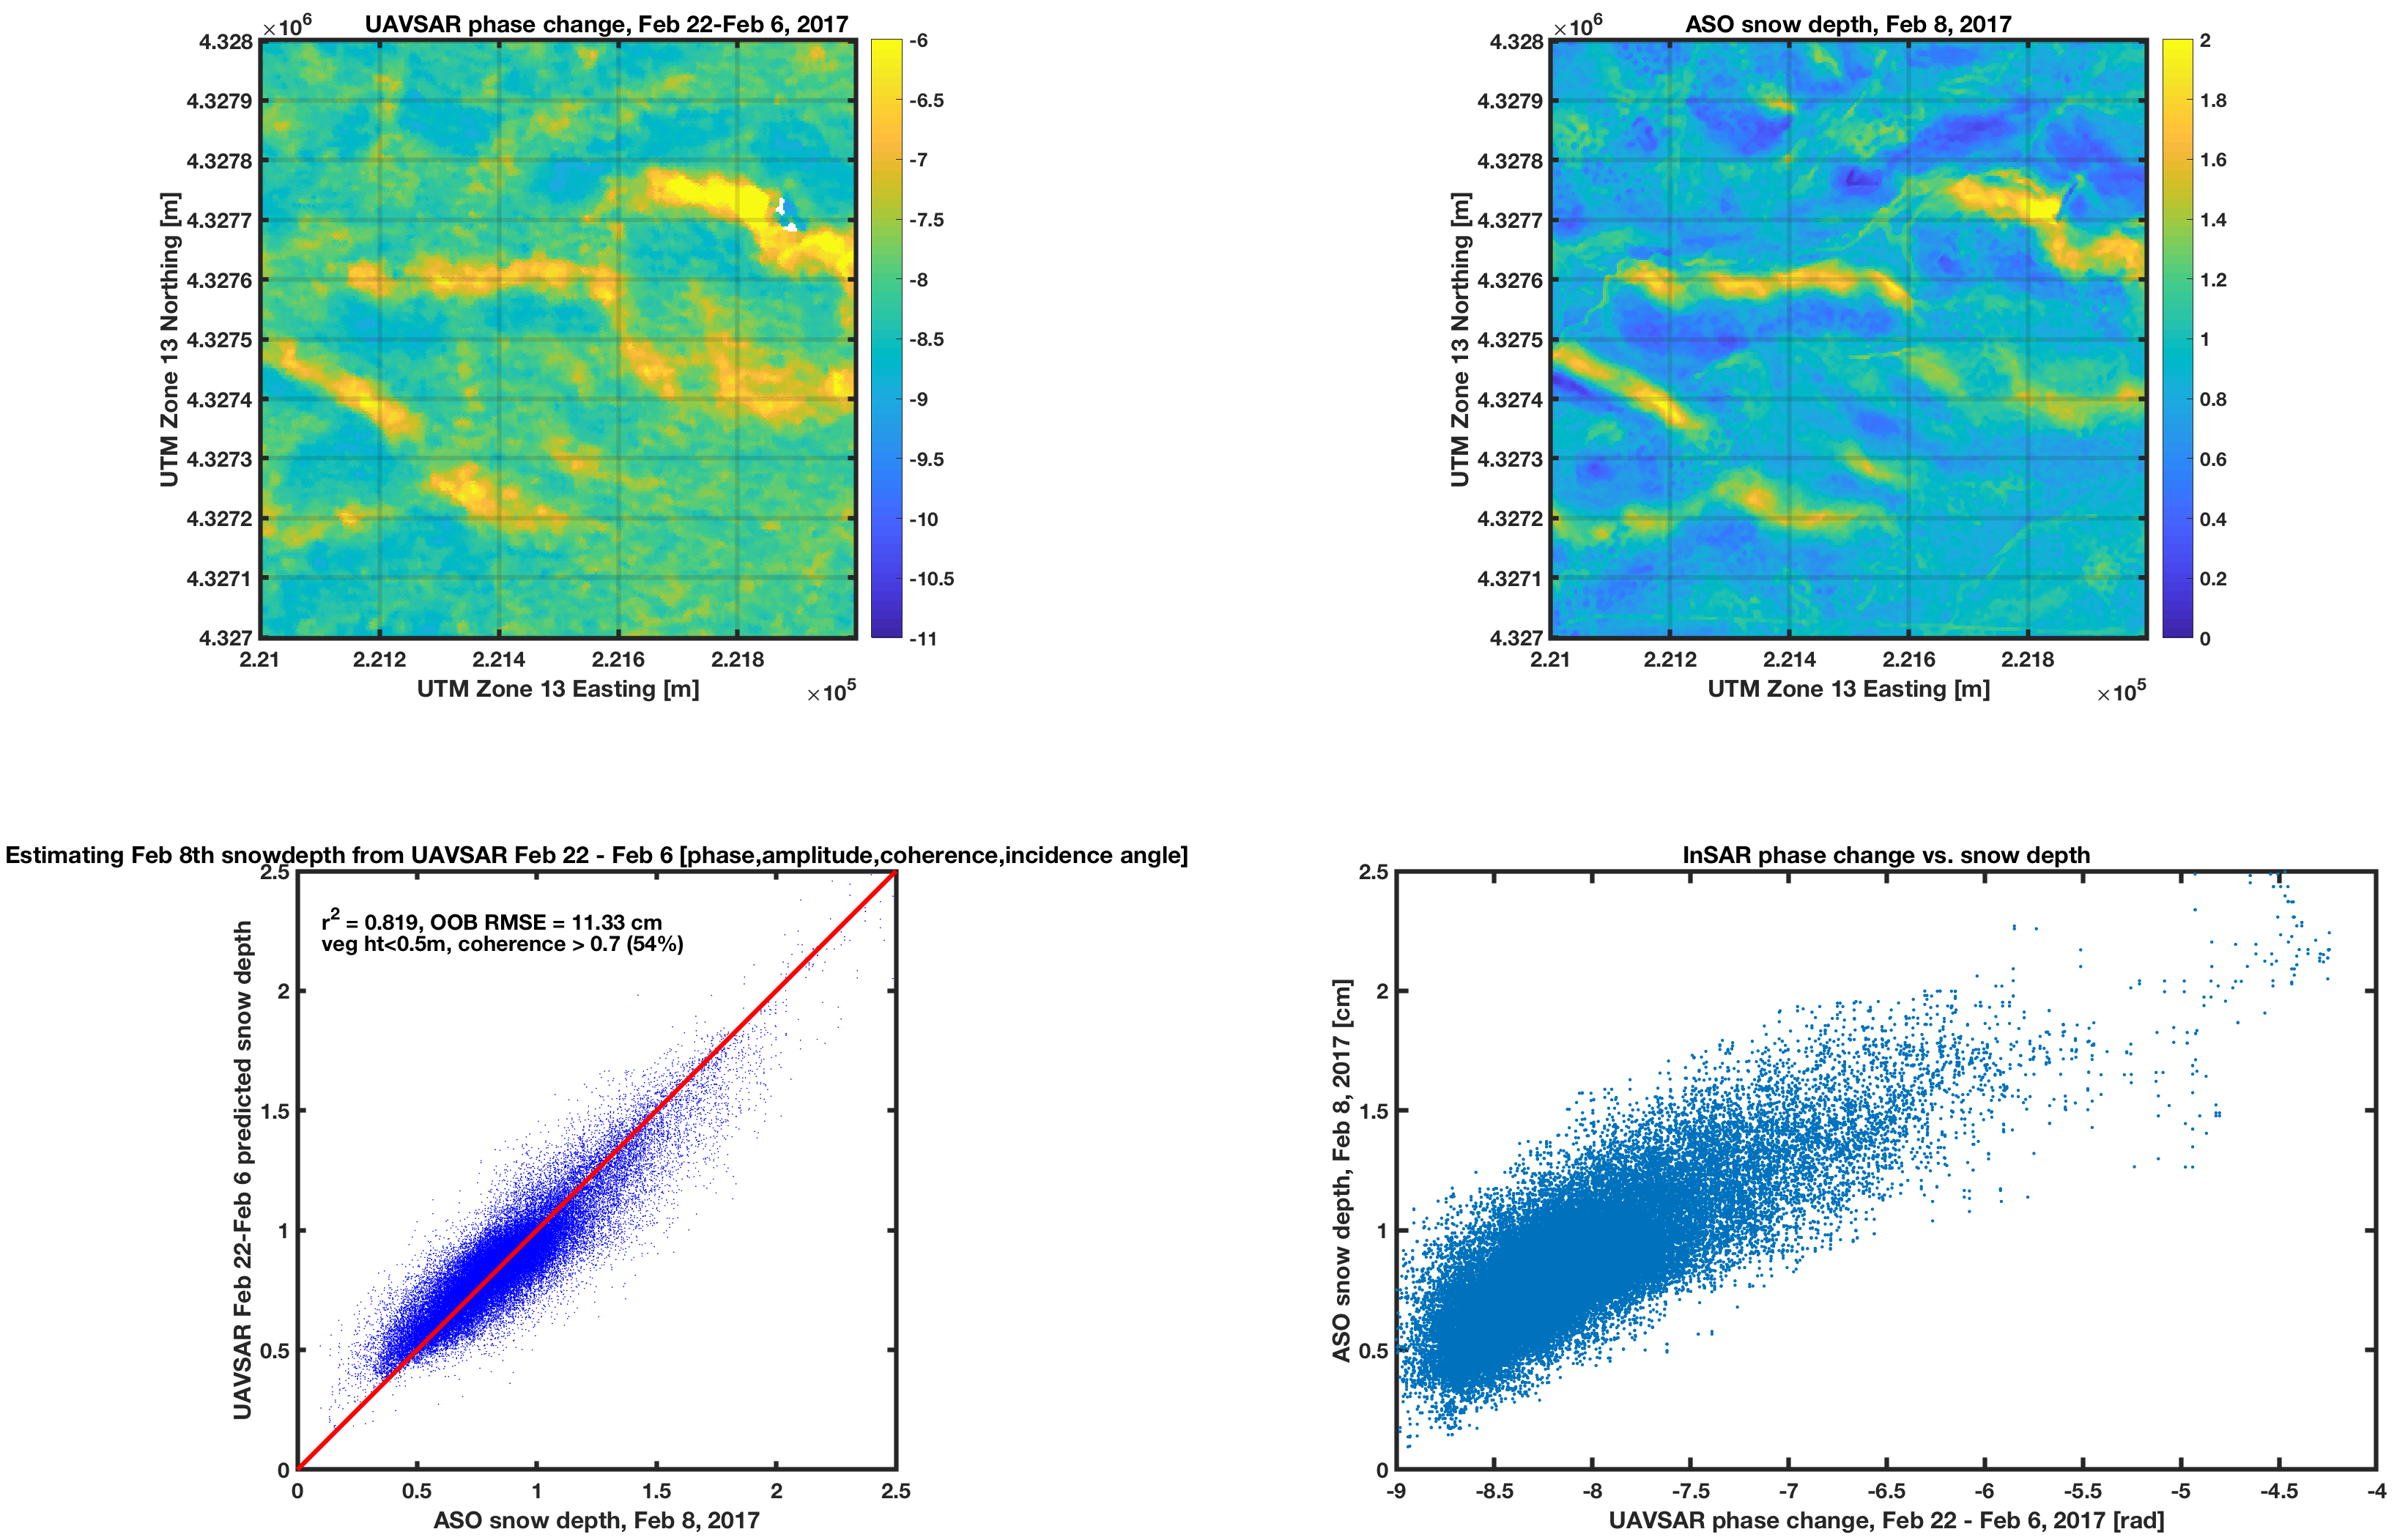
\includegraphics[width=1\columnwidth]{UAVSAR-ASO-GM2017_1km.png}
\caption{\small{Upper left: InSAR phase change [rad]. Upper right: LiDAR snow depth [m]. Lower left: predicted snow depth from random forest.  Lower right: InSAR phase change vs. LiDAR snow. depth }}
\label{fig:InSAR_LiDAR_1km} 
\end{figure}
\end{minipage}

}
\end{mysection}

\begin{mysection}{Depth change and total depth, compared to in-situ observations}
\vspace{-1cm}
\large{
\begin{itemize}
\item  LiDAR snow depths agree with in-situ observations with RMSE=10-20cm, as expected from previous studies
\item InSAR depth changes from \citet{Guneriussen:2001}:  \\ $\Delta d = -\frac{\Delta \phi \, \lambda}{4 \pi} \, \, \frac{1}{\cos{\alpha}-\sqrt{\epsilon_s - \sin^2{\alpha}}}$
\item Field campaign was designed to measure \textit{total SWE} distribution, not changes in SWE
\item Comparison with in-situ observations challenged by small total change (~10-20 cm) relative to short length scale variation (~30-50cm)
\item Changes in depth below accuracy of LiDAR, challenging the use of repeat snow-on LiDAR to map depth changes during February 2017
\end{itemize}

\begin{minipage}{1\columnwidth}
\begin{figure}
\centering
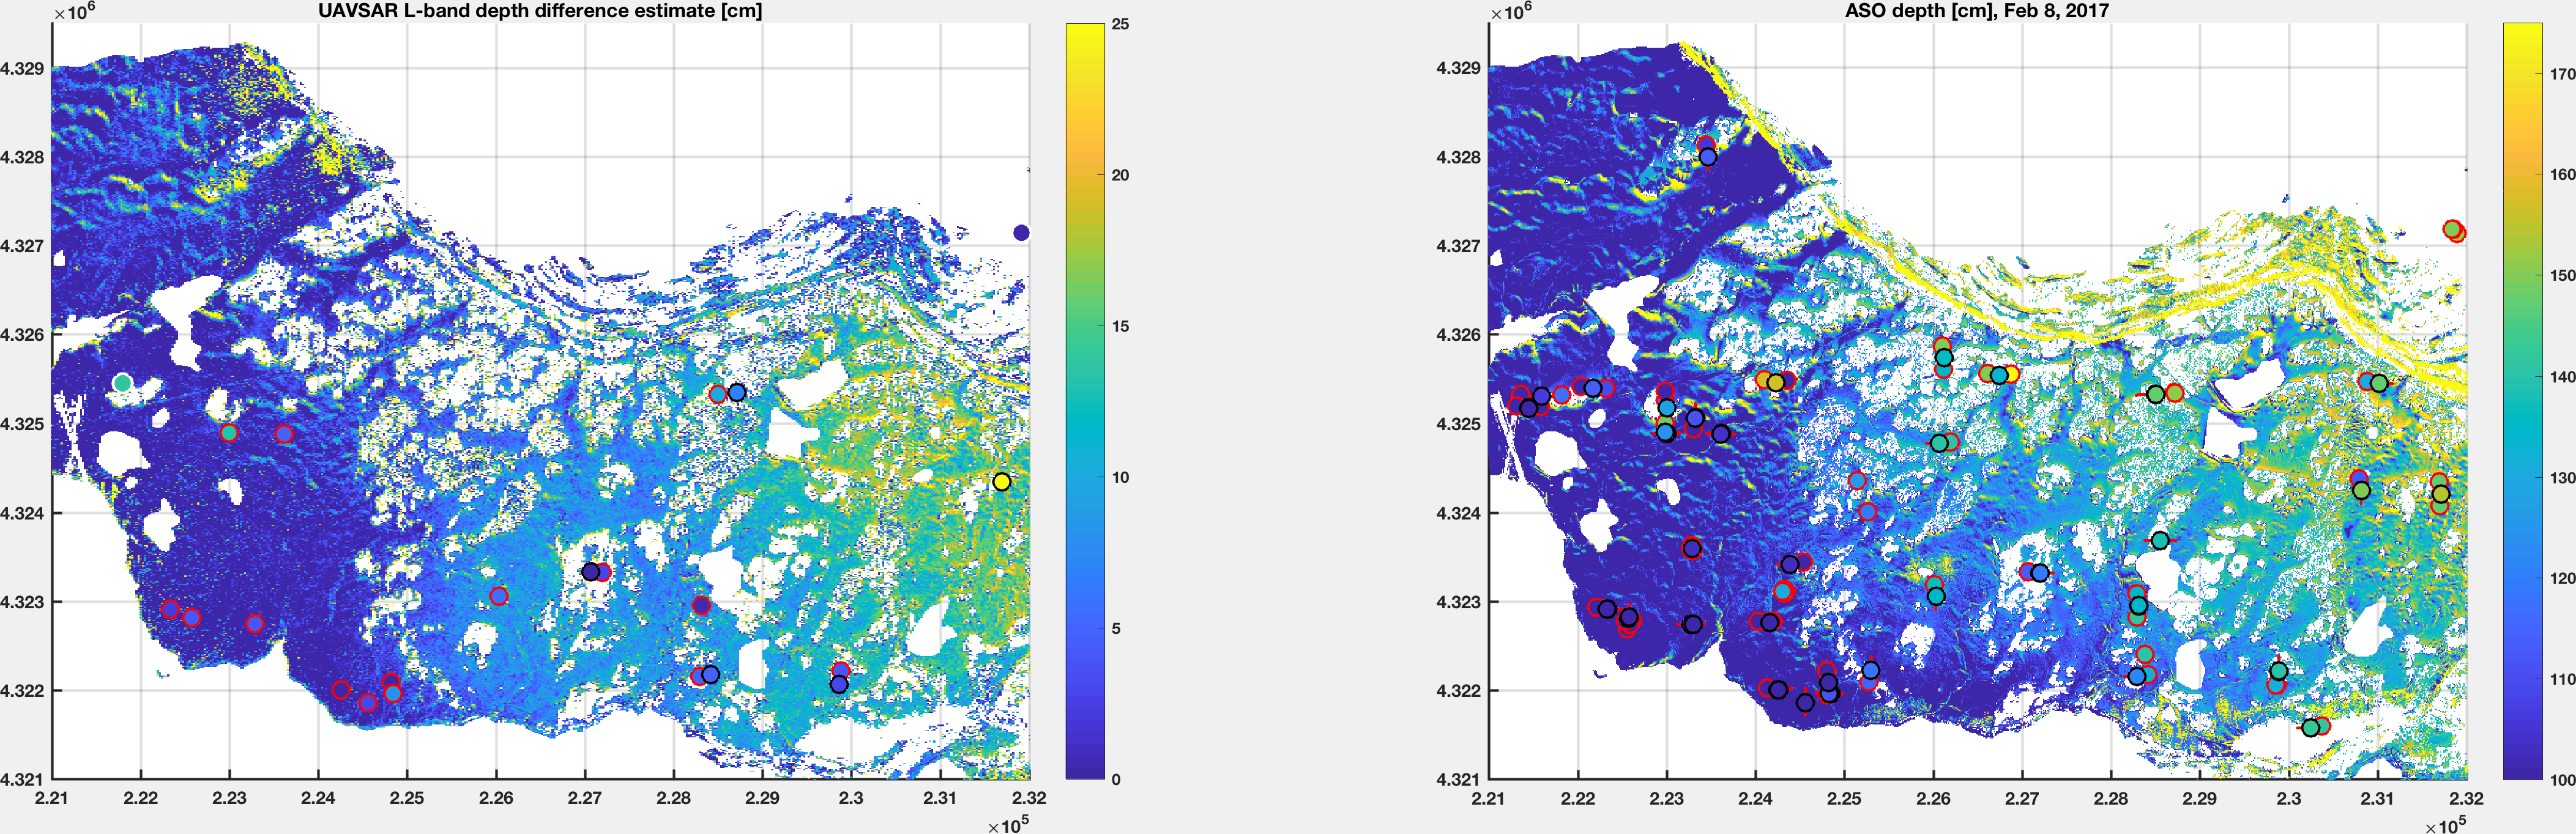
\includegraphics[width=1\columnwidth]{Fig8.png}
\caption{\small{Left: InSAR depth estimate, with in-situ depth changes shown with filled circles.  Right: LiDAR snow depth, with in-situ depths shown with filled circles.}}
\label{fig:InSAR_LiDAR_1km} 
\end{figure}
\end{minipage}

}
\end{mysection}
\begin{mysection}{InSAR depth change at 1 km$^2$ scale}
\vspace{-1cm}
\large{
\begin{itemize}
\item  At 1 km$^2$ scale in open region with large short length scale variability, InSAR depth changes mimic total snow depth pattern
\item  Over this region, LiDAR depth changes are reasonable, with the exception of a flight line artifact on the right side
\item  Depth changes from LiDAR and InSAR agree with an RMSE of 6.6 cm over a dynamic range of 25 cm, with a bias-corrected RMSE of 5.0 cm
\item  These depth changes correspond to SWE changes on the order of 1-4 cm, with an accuracy of less than 1 cm
\item  Sensitivity to new snowfall at the 1 cm level could be very useful to the snowfall remote sensing community 
\end{itemize}

\begin{minipage}{1\columnwidth}
\begin{figure}
\centering
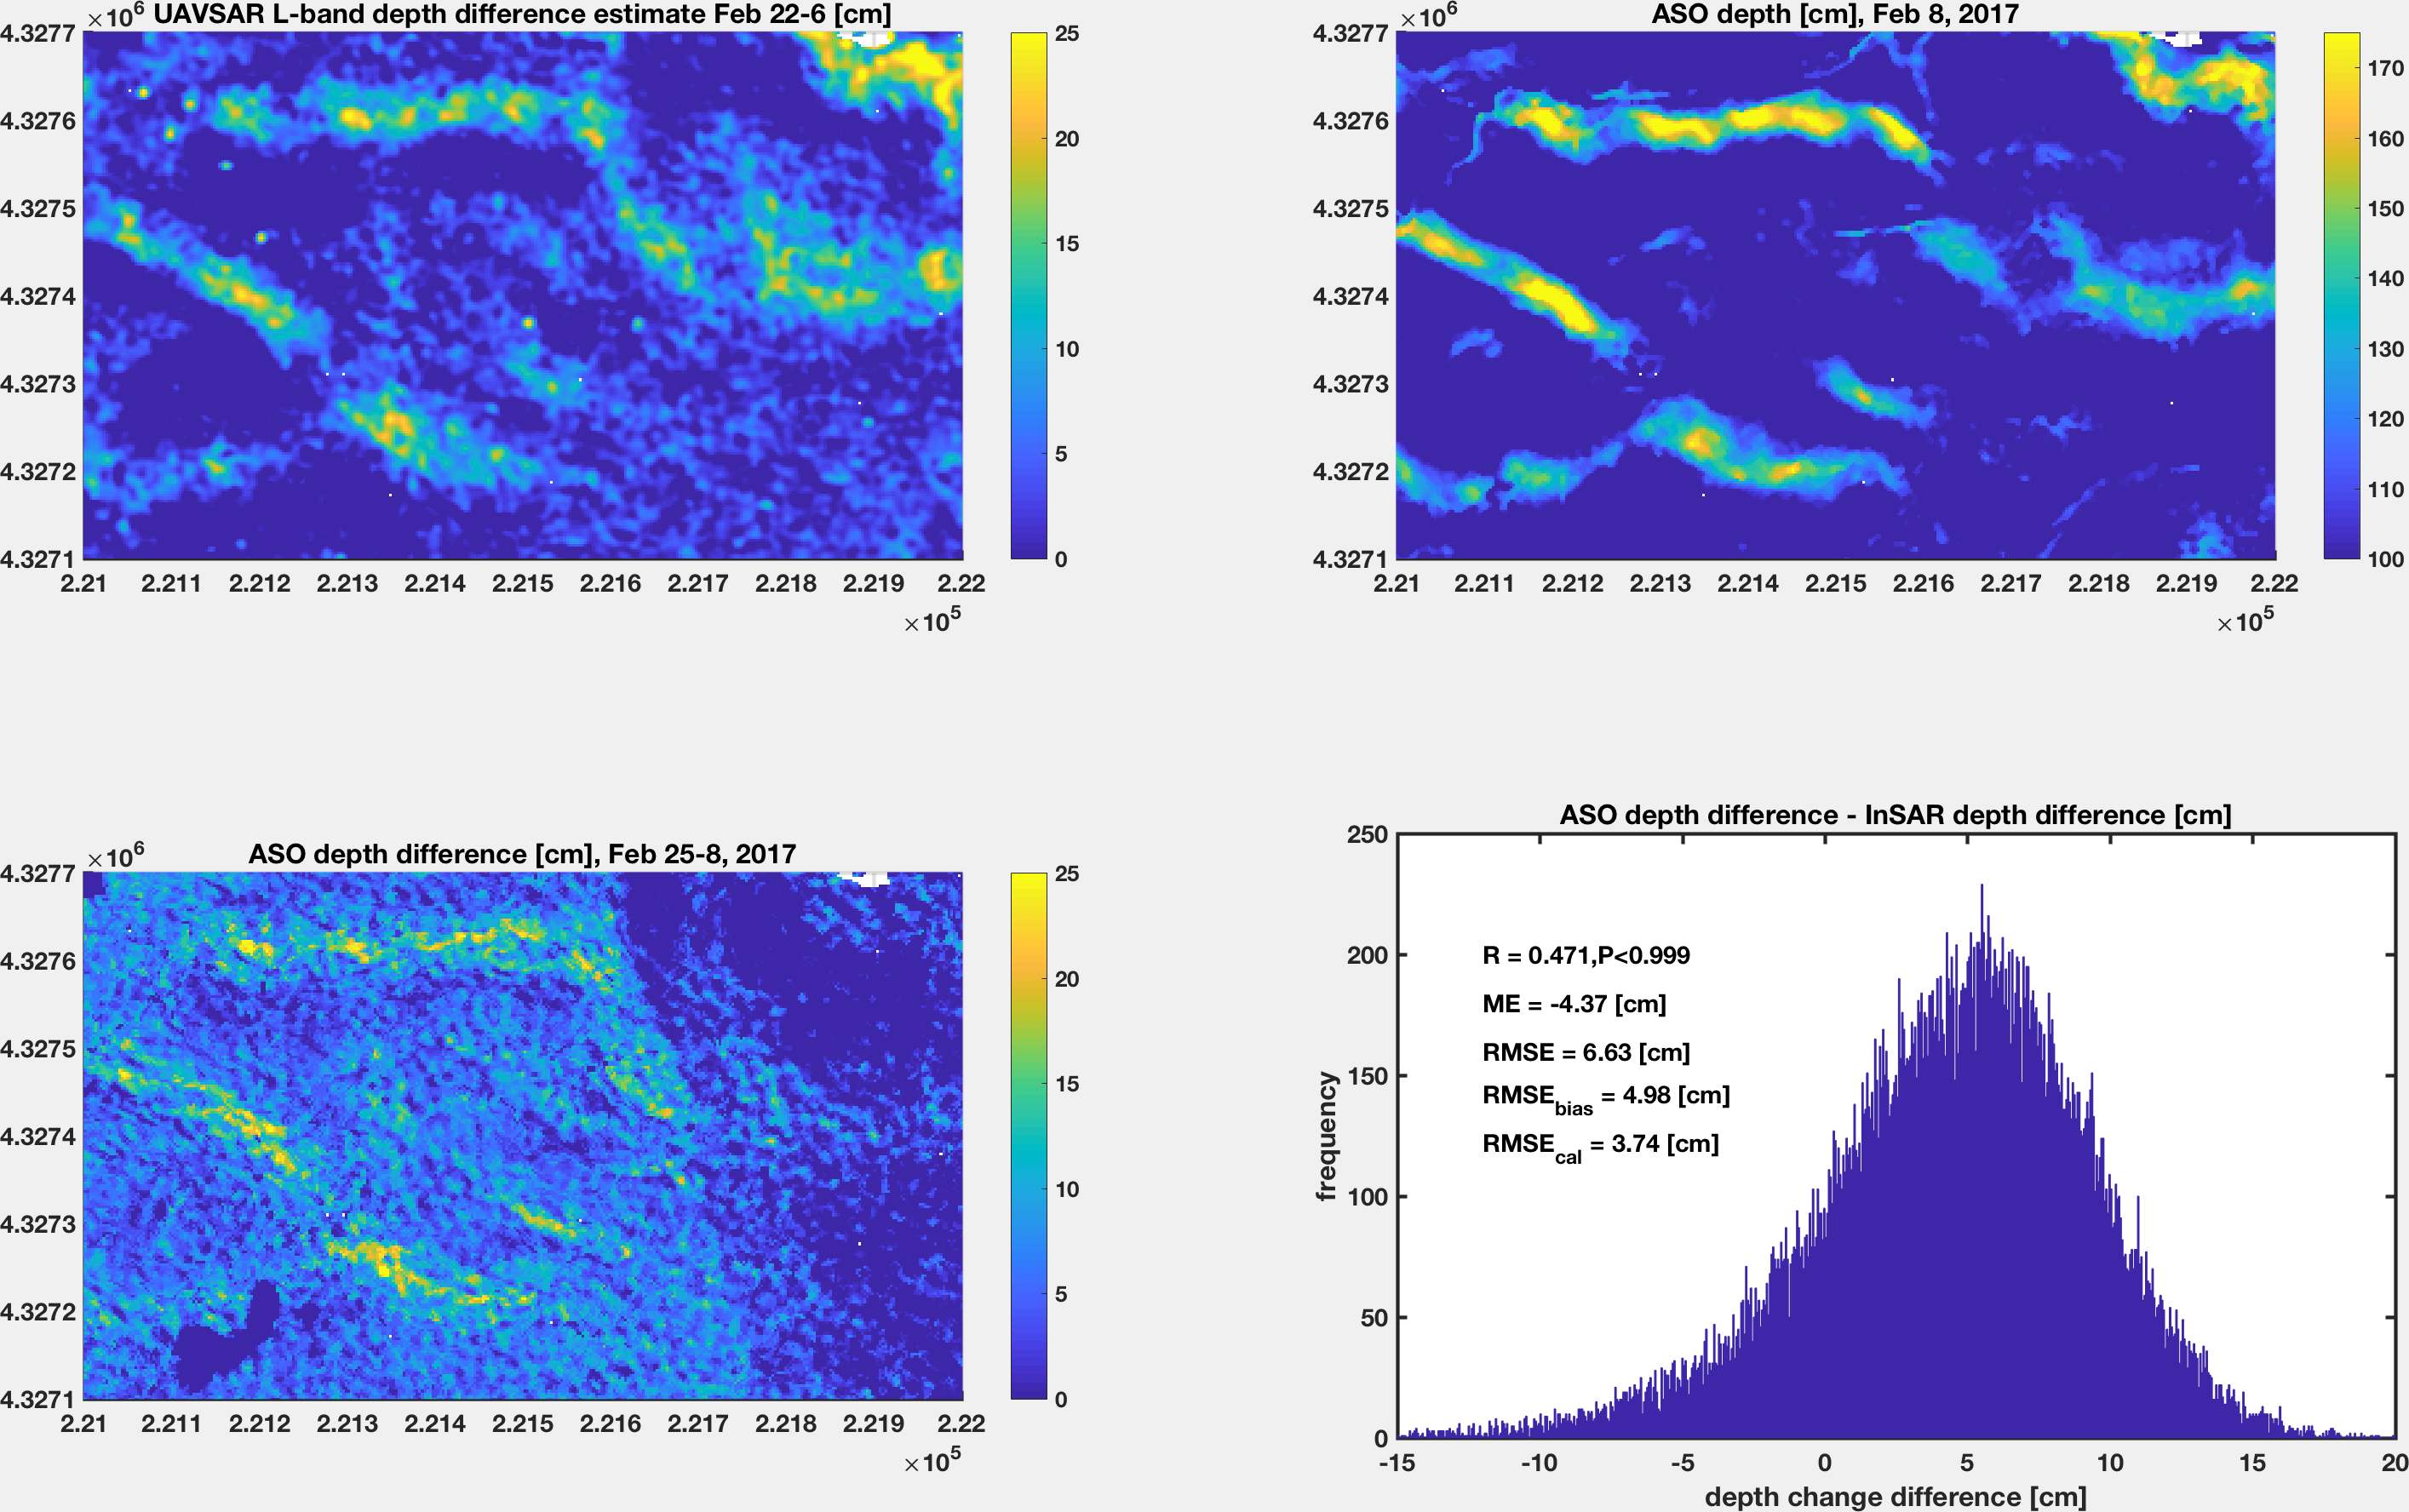
\includegraphics[width=1\columnwidth]{Fig9.png}
\caption{\small{Top left: InSAR depth change retrieval. Top right: LiDAR snow depth.  Bottom left: LiDAR depth change.  Bottom right: histogram of LiDAR-InSAR depth change.}}
\label{fig:InSAR_LiDAR_1km} 
\end{figure}
\end{minipage}

}
\end{mysection}


%\large{
%\begin{minipage}{0.6\columnwidth}
%\begin{figure}
%  \begin{center}
%   \includegraphics[width=1\columnwidth]{FMCWinsitu.pdf}
%   \caption{\small{Snowpit observations, In-situ reflectivity, FMCW profile, metal reflector exp}}
%   \label{fig:multiGPR} 
%  \end{center}
% \end{figure}
%\end{minipage}
%\begin{minipage}{0.35\columnwidth}
%\begin{figure}
%  \begin{center}
%   \includegraphics[width=1\columnwidth]{Reflectivity.png}
%   \caption{\small{In-situ reflectivity vs. FMCW backscatter}}
%   \label{fig:multiGPR} 
%  \end{center}
% \end{figure}
%\end{minipage}
%
%\begin{minipage}{0.4\columnwidth}
%\begin{figure}
%  \begin{center}
%   \includegraphics[width=1\columnwidth]{InSitu.png}
%   \caption{\small{In-situ dielectric constant}}
%   \label{fig:multiGPR} 
%  \end{center}
% \end{figure}
%\end{minipage}
%\begin{minipage}{0.3\columnwidth}
%\begin{figure}
%  \begin{center}
%   \includegraphics[width=1\columnwidth]{Layers.png}
%   \caption{\small{Arctic snow stratigraphy}}
%   \label{fig:multiGPR} 
%  \end{center}
% \end{figure}
%\end{minipage}
%\begin{minipage}{0.3\columnwidth}
%\begin{figure}
%  \begin{center}
%   \includegraphics[width=1\columnwidth]{LayerVar.png}
%   \caption{\small{Layer variation in three parallel trenches over 50cm}}
%   \label{fig:multiGPR} 
%  \end{center}
% \end{figure}
%\end{minipage}
%
%\begin{minipage}{0.65\columnwidth}
%\begin{itemize}
%\item Continuous reflections caused by density changes at layer boundaries
%\item Cause of reflections can be confirmed with metal reflection experiments
%\item Amplitude of reflection is a function of dielectric contrast
%\item Small scale variations in stratigraphy larger than variations in bulk properties
%\item Average reflectivity and average radar backscatter from layer boundaries highly correlated
%\end{itemize}
%\end{minipage}
%\begin{minipage}{0.3\columnwidth}
%\begin{figure}
%  \begin{center}
%   \includegraphics[width=1\columnwidth]{MuliGPR.pdf}
%   \caption{\small{Multi-channel radar for continuous density profiling}}
%   \label{fig:multiGPR} 
%  \end{center}
% \end{figure}
%\end{minipage}
%
%}
%\end{mysection}

%%% Conclusions %%%
%\begin{mysection}{Conclusions}
%\large{
%\begin{itemize}
%\item Variations below 500 m can be large, and high resolution observations at the km-scale are needed to understand and model snow distribution accurately
%\item High resolution (2cm vertical, 10cm horizontal) radar measurements produce detailed view of spatial distribution of depth, density, stratigraphy and density profiles at a resolution and scale not possible with traditional techniques.  
%\item Measurements at the km scale are quick and low cost, and bridge the gap between point observations and remote sensing and modeling pixel scales.
%\item Amplitude of reflections from layer boundaries are highly correlated with magnitude of density change, but require averaging many observations
%\item Multi-channel radar allows independent measurements of layer thickness and density
%\item Combining multi-channel radar with forward modeling = accurate profiles of density, layer boundaries, liquid water content 
%\end{itemize}
%
%\begin{minipage}{0.4\columnwidth}
%\begin{figure}
%  \begin{center}
%   \includegraphics[width=1\columnwidth]{DoubleRadar.jpg}
%   \label{fig:SMP_profile} 
%  \end{center}
% \end{figure}
%\end{minipage}
%\begin{minipage}{0.3\columnwidth}
%\begin{figure}
%  \begin{center}
%   \includegraphics[width=1\columnwidth]{HPAndyRadar.jpg}
%   \label{fig:SMP_profile} 
%  \end{center}
% \end{figure}
%\end{minipage}
%\begin{minipage}{0.3\columnwidth}
%\begin{figure}
%  \begin{center}
%   \includegraphics[width=1\columnwidth]{radar2.jpg}
%   \label{fig:SMP_profile} 
%  \end{center}
% \end{figure}
%\end{minipage}
%}
%\end{mysection}


\begin{mysection}{Acknowledgments}

\small{
This work was funded by the NASA Terrestrial Hydrology Program, grant \#NNX17AL61G, NASA JPL subcontract \#1580367, and U.S. Army CRREL.

\nocite{Deeb:2011,Engen:2004,Li:2017}

\vspace{-2cm}

\bibliography{snow_2018}
}
\end{mysection}



\end{multicols}
  
%\begin{multicols}{2}
%\begin{mysection}{Km-scale profiles}
%\large{
%\begin{minipage}{0.6\columnwidth}
%\begin{figure}
%  \begin{center}
%\includegraphics[width=1\columnwidth]{SBB.png}
%\caption{\small{2-10 GHz FMCW radar measurements in the high alpine, Senator Beck Basin, CO.}}
%\label{SBB} 
%\end{center}
%\end{figure}
%\end{minipage}
%\begin{minipage}{0.3\columnwidth}
%\begin{figure}
%\begin{center}
%\includegraphics[width=1\columnwidth]{SBB2.pdf}
%\caption{\small{Map of radar profiles in Senator Beck Basin.}}
%\label{SBTOP} 
%\end{center}
%\end{figure}
%\end{minipage}
%
%\begin{figure}
%\includegraphics[width=0.95\columnwidth]{LiDAR-Scale-Resolution5.pdf}
%\caption{\small{Why high resolution matters: details at scales less than 500m are often complex, complicating ground-truth of remote sensing footprints at this scale.}}
%\label{fig:LiDARres} 
%\end{figure}
%}
%\end{mysection}
%\end{multicols}
\end{poster}

\end{document}

